\subsection{The Idea of a Class}

§1 \quad Set theory builds much from remarkably little. Starting from pure logic and a single fundamental relation, it can represent ordered pairs, relations, functions, numbers, spaces, and much of the ordinary machinery of mathematics. By encoding all of this into a unified language, set theory serves as a rigorous foundation for the discipline as a whole.

§2 \quad At the same time, set theory is the mathematical theory of infinity in its own right. It studies infinite collections directly: what kinds of infinities there are, how their sizes can be compared, and how far the universe extends beyond the finite. 

§3 \quad To achieve all of this, the theory employs a minimal vocabulary. We speak of objects, called \textit{classes}, and we take as primitive a single relation between them: the relation of \textit{membership}, symbolized by $\in$. Thus, $x \in A$ says that the class $x$ is a member of the class $A$. The relation $\in$ is not defined in terms of anything more basic. Rather, it is the primitive starting point from which the rest of the theory is built.

§4 \quad In a first pass, a class is simply a collection: something of which objects may be members. Later, we shall distinguish carefully between classes that are \textit{sets} and classes that are too large to be sets. Roughly, sets are the classes small enough to be members of other classes. This distinction will be one of the first real lessons of the theory.

§5 \quad It may feel unsatisfying that we cannot define what a class or membership \textit{is} in some more basic vocabulary. Because they are our absolute starting points, strict mathematical definition is impossible. Instead, we must rely on intuition, triangulating the concept using three distinct but supplementary routes that all lead to the same underlying idea. 

§5.1 \quad The first route is psychological: the everyday act of gathering distinct things together to treat them as a single object of thought. When we speak of the Beatles, for instance, we take John, Paul, George, and Ringo, and conceptually unite them into a single entity. The individuals do not physically merge, nor do they lose their separate identities, yet we effortlessly grasp the band as one collective whole. Set theory starts from this pure intellectual gesture: the decision to consider the many as one.

§5.2 \quad The second route is spatial: the image of containment. We instinctively picture the members of a class as lying ``inside" a boundary that gathers them together. 

\begin{figure}[h]
\centering
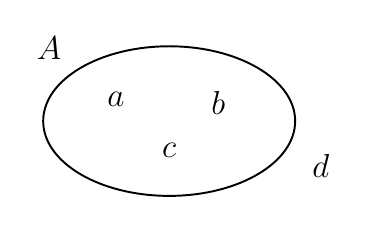
\begin{tikzpicture}[x=0.5cm,y=0.5cm]
    % The class A
    \draw[line width=0.7pt] (0,0) ellipse (3.2 and 1.9);
    \node[font=\large] at (-3.05,1.85) {$A$};

    % Members of A
    \node[font=\large] at (-1.35,0.55) {$a$};
    \node[font=\large] at (1.25,0.45) {$b$};
    \node[font=\large] at (0,-0.75) {$c$};

    % An object not belonging to A
    \node[font=\large] at (3.85,-1.15) {$d$};
\end{tikzpicture}
\caption{The objects $a$, $b$, and $c$ are members of $A$, while $d$ is not.}
\end{figure}

§5.3 \quad The third route is structural, moving away from physical space and toward formal symbols. Set theory typically gathers objects using \textit{brace notation}. We write $\{a,b,c\}$ for the class whose members are exactly $a$, $b$, and $c$. This notation highlights a subtle shift in thought: $a$ is an object, while $\{a\}$---called the \textit{singleton} of $a$---is the formal ``container" holding that object. A class is not a physical box, and its members are not material parts lying inside it; rather, membership is a matter of \textit{formal} belonging.

§6 \quad These three perspectives---the unified whole, the spatial boundary, and the formal container---all circle the same primitive reality. We can capture this shared intuition in an explicit, though strictly informal, definition.

\begin{definitionzero}[Informal]
A \textit{class} is a single mathematical object formed by treating specific objects together as a unified whole.

For any class $x$ and any class $A$, we write 
\[x \in A,\] 
read as ``$x$ is an \textit{element} of $A$,'' or ``$x$ \textit{belongs to} $A$'',
to express the primitive fact that $x$ is one of the objects participating in that unified whole.
\end{definitionzero}

§7 \quad Once the primitive relation $\in$ has been introduced, we can define its negation. We write that $x \notin A$ iff it is not the case that $x \in A$. Thus, $\notin$ is not a second primitive relation, but an abbreviation defined in terms of membership and logic. In symbols:
\[
x \notin A \quad := \quad \neg(x \in A).
\]
Looking back at our diagram and brace notation, we can now formally write that $a \in A$ and $a \in \{a,b,c\}$, while $d \notin A$ and $d \notin \{a,b,c\}$.

§10 \quad There is a subtle danger, however, in trusting these intuitive routes too completely. By writing $\{a,b,c\}$, or by drawing a boundary around them and calling it $A$, we make it look as though such a class has already been successfully secured. But notation and pictures do not \textit{create} classes. They merely allow us to describe a possible collection; they do not by themselves bring such a collection into existence. 

§11 \quad This is why set theory needs laws that say which collections may exist, which collections count as sets, and which operations on sets are legitimate. Without such laws, the idea of forming a collection based purely on intuition is too permissive. As we will soon see, unrestricted collection leads to paradox. Membership becomes mathematically powerful only once it is governed by rules. These rules will be given in the form of axioms.